\documentclass[12pt,letterpaper]{article}
\usepackage{amsmath,amsthm,amsfonts,amssymb,amscd}
\usepackage{fullpage}
\usepackage{lastpage}
\usepackage{enumerate}
\usepackage{fancyhdr}
\usepackage{tikz}
\usetikzlibrary{arrows, automata}
\usepackage{mathrsfs}
\usepackage{dsfont}
\usepackage[margin=3cm]{geometry}
\setlength{\parindent}{0.0in}
\setlength{\parskip}{0.05in}
\usepackage{caption}
\usepackage{subcaption}
\usepackage{float}

\newcommand\refobj{\textmd{ref}}
\newcommand\tab[1][1cm]{\hspace*{#1}}
\newcommand\prob{\mathbb{P}}
\newcommand\E{\mathbb{E}}
\DeclareMathOperator*{\argmin}{\arg\!\min}
\title{Grounding Language to Exact Locations}

\begin{document}
\maketitle
\section{Introduction}

\subsection{The Problem}

\tab In Grounded-Language Applications for Robotics, natural language is usually talked about as referring to important \textbf{objects} in the robot's visual field (Tellex 2011). However, natural language can also refer to \textbf{locations} in relation to a reference object. This kind of referential expression is composed of a relation and a reference object. For example, `to the right of the banana' is a referential expression, with `right' as the relation and `the banana' as the reference. In this paper, we develop NLP algorithms that might give robots the ability to understand these locational referential expressions.\\
\tab In English, \textbf{exact locations} are referred to using measurement phrases (``five inches", ``one foot") which co-occur with prepositional phrases like ``to the right of X" and ``to the left of X". Our program would allow us to parse statements such as ``five inches left of the car". Essentially, our program provides a way for robots to interpret an answer the question: \textit{where? Where is the new object I haven't scanned for yet? Where should I put this object down? Where has this object been moved to?}\\
\tab The inputs to our program are a \textbf{command}, natural language spoken by the user, as well as the \textbf{world}, which consists of the \textbf{table} \--- the region where points can lie (literally a ``table") \--- its \textbf{dimensions}, \textbf{objects} on the table, and \textbf{walls} (the edges of the table). Our output is a probability distribution around (x,y) coordinates on the table. Our goal is to develop an algorithm that can understand where humans actually mean when they utter these phrases. That is, to estimate:

\[\prob((x,y) | command, world)\]

We specify a distribution rather than an ``exact point" because humans themselves do not behave uniformly when referring to these locations. In linguistic terminology, these expressions are vague. To give the reader the intuition, the utterance ``5 inches left of the car" could be referring to any point that is 5 inches extending out from the left side of the car, but humans can choose from what point on the car to extend: this problem we call the problem of how to pick a \textbf{reference point}. Even more broadly, humans can choose to interpret ``left" as relative to the speaker, themselves, or relative to the car itself: humans can choose different \textbf{frames of reference} (Levinson 2001). For our purposes, the \textbf{relative frame of reference} is relative to the robot, and the \textbf{intrinsic frame of reference} is relative to the reference object's intrinsic left/right/front/back (Levinson 2001). To uncover these particular kinds of issues, we performed an experiment on humans discussed below. This experiment also allowed us to establish a human baseline with which to evaluate our algorithms.\\
\tab Moreover, a distribution is helpful for future practical applications of our algorithm. For example, if a human moves an object and tells the robot ``it is 5 inches left of the car", the robot will want to scan intelligently in a particular area surrounding that point. Without a distribution, it only has the point itself to rely on. 

\subsection{Previous Research}

\tab Researchers in the Humans to Robots lab are improving Baxter's ability to interact with humans and refer to objects in Baxter's workspace, and much of their research is extremely relevant to our project. Currently, Baxter can pick up objects that are directly referred to with voice commands, such as ``give me the wooden bowl."  Emily Wu is developing social feedback mechanisms based on language grounding, Advik Guha is determining object placement in a discrete grid with POMDPs, and Gaurav Manek is developing a object-detection parser using natural language prepositional phrases. Although Guha's work specifies locations, he focuses on robot action, using a limited language parser that does not include reference to exact locations through speech (he mostly uses pointing). Our algorithm adds the ability to numerically specify locations relative to reference points. Although Gaurav builds an intelligent parser that encompasses a wide range of locational features and words (like ``between", ``above", ``to the left of", ``in front of"), he uses it to predict groundings of particular objects, not locations in space. We plan to bridge these two different projects: to build an intelligent natural-language observation function that specifies locations in space (without corresponding actions).

\subsection{Practical Implications}

Our program has many applications, some of which are enumerated below:

\begin{enumerate}[(1)]
\item lets the user interact with the robot in placing tasks
\item allows the user to specify a new location of an object if the object has moved
\item allows the user to set waypoints that the robot could use for further tasks: e.g. if a user wanted to use a particular location in space that the robot could not detect using vision 
\end{enumerate}

Specifying spatial locations is an important problem that humans can solve, and would generalize into many other tasks in robotics. 

\subsection{Roadmap}

\textbf{Section 2} discusses our experiment that provided a human baseline for training and testing our algorithms. \textbf{Section 3} presents a log linear model that creates a distribution over spatial coordinates given a command and world. There we derive four features of the model use MLE estimation to find their weights. \textbf{Section 4} evaluates this model with different features turned on and off. \textbf{Section 5} discusses extensions of our model currently being worked on, as well as future research. \textbf{Section 6} concludes.

\section{Human Experiment}

\subsection{Goal}

The overarching goal of our experiment was to figure out exactly how humans interpreted these expressions. We assume that humans use these expressions in the same way that they interpret them: users would want the robot to interpret their expression like a human being would. Thus, the robot can learn how to interpret these expressions by learning from human data. For practical purposes, this data helps us in two ways:

\begin{enumerate}[(1)]

\item Provides \textbf{training} \textbf{data} that tells us what kinds of features are important to include in our algorithms.\\
\item Provides \textbf{testing} \textbf{data} to evaluate the accuracy of different algorithms.
\end{enumerate}

We used a preliminary experiment, similar to the following one, to inform the following experiment and to get a sense of what worked. In this more developed experiment, we used two scenes to inform the construction of our algorithm, and two scenes to test our algorithm on.

\subsection{Method}

Setup for our experiment consisted of a 3x4-foot whiteboard, on which three objects were taped. Subjects were prompted with twelve commands referring to points on the whiteboard relative to the objects; for each command, they placed a dot on the point on the whiteboard that they thought the expression referred. Each command was of the following form, and drawn from the sets below:\\

\noindent \textbf{Number} \tab	\textbf{Measurement}	 \tab	\textbf{Relation} \tab		\textbf{Object}\\
five		\tab \tab  	inches	\tab\tab\tab   	behind	\tab	 	the car\\

\noindent \textbf{Number}: Any positive integer, optionally plus $1/2$ \\
\textbf{Measurement}: inch, inches, foot, feet\footnote{Our preliminary experiment told us that American subjects were horrible at estimating centimeters, and would probably never use the metric system in actual speech.}\\
\textbf{Relation}: ``(to the) left of", ``(to the) right of", ``in front of", ``behind"\\
\textbf{Object}: ``the lid", ``the keyboard", ``the car", ``the pink bowl"\\

For our purposes, the \textbf{world} consists only of the whiteboard as a two dimensional object. The \textbf{walls} in this setup were the sides of the whiteboard, and the \textbf{objects} were the three objects taped to it in each experiment.\\
\tab Our preliminary experiment told us that certain expressions like ``in front of" and ``behind" are interpreted differently when the whiteboard is placed at different heights. Therefore, the whiteboard was elevated at a consistent height to mimic the \textbf{table} on which Baxter sits in the H2R Lab. This way, a human would interact with the white board in the same way Baxter would.\\
\tab A picture of the outcome of a particular experiment is below:
\begin{figure}[H]
\centering
\includegraphics[scale=.1]{"images/scene1"}
\caption{Outcome of one trial of the experiment. Points are numbered with the corresponding command number to allow us to collect data afterwards.}
\label{fig:experiment}
\end{figure}
\tab There were four scenes, each with different configuration of objects and different commands. Scene 1 and 2 involved no rotation of the large object (the lid/keyboard); scene 3 and 4 involved rotation of the lid/keyboard. Information about these scenes shown in the following table: \\


\begin{tabular}{c c c c c}

 & Number of Subjects & Number of Commands & Train/Test & Rotated Objects?\\
\hline
Scene 1 & 11 & 12 & Train & No\\
Scene 2 & 11 & 12 & Test & No\\
Scene 3 & 11 & 12 & Train & Yes\\
Scene 4 & 10 & 12 & Test & Yes
\end{tabular}


\subsection{Results}

Results from this experiment were informative in many ways, enumerated below:

\begin{enumerate}[(1)]
\item Points were measured from edge of the object (as opposed to its center)
\item Variance appears to scale linearly with distance
\begin{figure}[H]
\centering
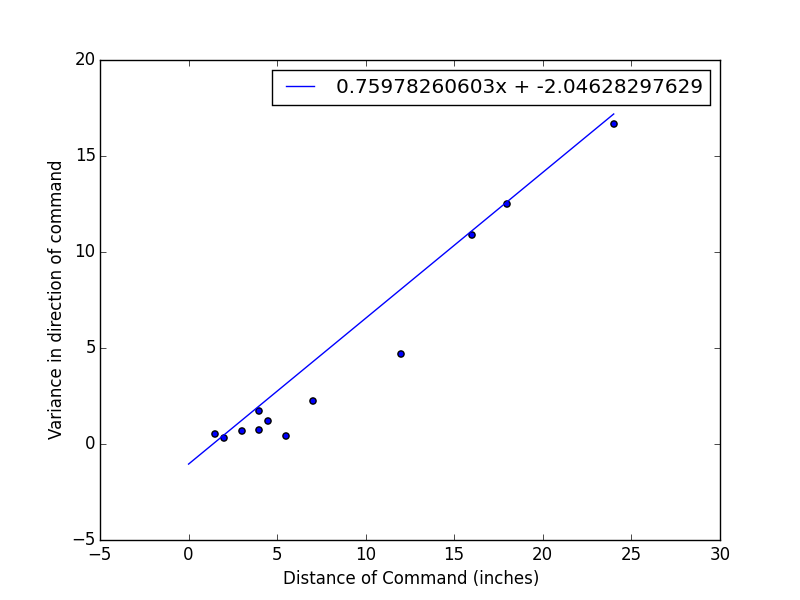
\includegraphics[scale=0.5]{images/varplot.png}
\caption{Plot of variance versus command distance}
\label{fig:varplot}
\end{figure}
\item Most subjects underestimated the point when objects fell in the path of the measurement, or the point was closer to another object than the one referenced in the command. That is, underestimated relative to their other estimations, and the ``real point" (measured with a ruler from the edge of the object)

\item Most subjects underestimated the point when walls fell in the path of measurement, or used an intrinsic frame of reference where they usually would have used a relative frame of reference.


\item \textbf{Frame of Reference}: Subjects always used relative frame of reference for Scene 1 and Scene 2. For rotation scenes (3 and 4), subjects usually used the relative frame of reference for ``left of" and ``right of", but occasionally used the intrinsic frame of reference for objects with intrinsic sides (the keyboard and the car). For ``in front of" and ``behind", subjects used both relative and intrinsic frames of reference, only intrinsic for the keyboard, the car and the lid. 

\item \textbf{Reference points}: Measurement extended from the center of the edge closest to the direction specified in the command OR from the point on the object that was maximally in the direction specified in the command. That is, there is broadly two kinds of ``reference points". As seen in Figure \ref{fig:refpts}, subjects used multiple reference points on the object as well as different frames of reference.

\begin{figure}[H]
\centering
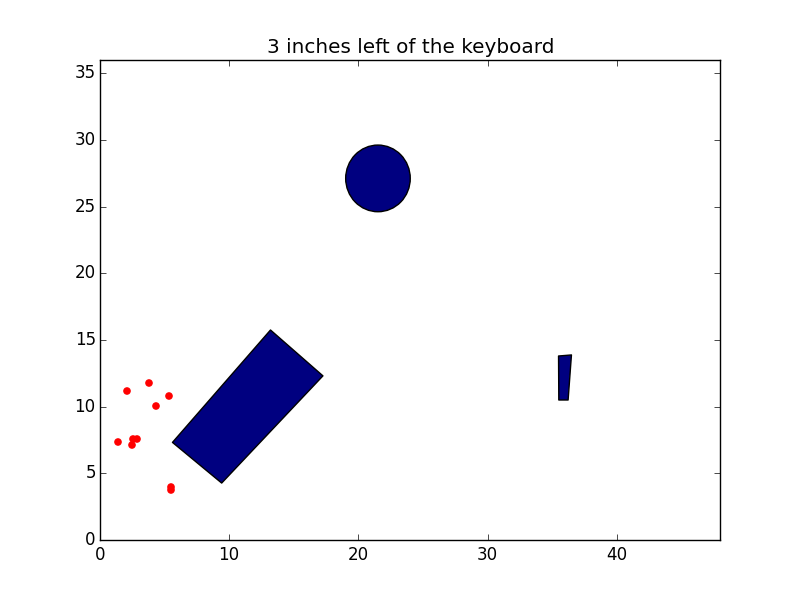
\includegraphics[scale=.5]{images/exp_3_cmd_11.png}
\caption{Experiment 3, Command 11}
\label{fig:refpts}
\end{figure}

\end{enumerate}

We address issues 1-4 in our algorithm below. We are currently in the process of developing an algorithm that takes into account 5 and 6, and seeing success.


\section{Mathematical Model}
Let $\Gamma$ represent the knowledge of the table. $\Gamma$ is composed of $\gamma_1, \ldots, \gamma_n$, corresponding to the objects on the table, and $\gamma_{\textmd{wall}_1}, \gamma_{\textmd{wall}_2}, \gamma_{\textmd{wall}_3}, \gamma_{\textmd{wall}_4}$, corresponding to the four walls (edges) of the table. Each $\gamma$ contains position and dimension information about the object in question.   \\
\\
Let $\lambda$ be the command the user gives, consisting of a distance $\lambda_d$ a direction (relation) $\lambda_r$ and a reference object $\lambda_f$. For the sake of testing this algorithm, we will assume perfect ability to parse the command and extract this information. Therefore we assume there is a perfect correspondence between $\lambda_f$ and $\gamma_\refobj$, where $\gamma_\refobj \in \{\gamma_1, \ldots, \gamma_n\}$. In addition, we assume that the direction is in the set $\{$left, right, in front, behind$\}$ and map $\lambda_r$ to the corresponding direction vectors $\{[1, 0], [-1, 0], [0, 1], [0, -1]\}$.  Underlying this assumption is the larger assumption that all commands map to a single direction vector - discussion of how we plan to improve this can be found later in this paper. We assume that the distance $\lambda_d$ of a command is independent of the direction $\lambda_r$. Finally, we only deal with two dimensions, so don't consider commands that involve the $z$-axis. \\
\\
As an example, if the command is `five inches to the right of the bowl', then we have $\lambda_d = 5$, $\lambda_r = [1, 0]$, $\lambda_f = $ the bowl. \\
\\
Our goal then is to estimate a function $\mathbb{P}(x, y | \lambda, \Gamma)$ which gives the probability that a user was referring to the point $(x, y)$ given the command $\lambda$ and world $\Gamma$. \\
\\
From the command and reference, we calculate a naive mean, which is the point you would select if you went exactly the distance specified by the command, in the direction specified by the command. From this we calculate four features for a log-linear model. 

\subsection{Feature Calculation}
\subsubsection{Calculating $\hat{\mu}$}
The naive mean, $\hat{\mu}$, is what is obtained by going exactly the distance specified in the command from the edge of the object. This is calculated as follows:
\[
\hat{\mu} = \begin{cases} 
\gamma_\refobj.center + \frac{1}{2}\gamma_\refobj.height + \lambda_d, & \lambda_r = [0, -1] \\
\gamma_\refobj.center - \frac{1}{2}\gamma_\refobj.height - \lambda_d, & \lambda_r = [0, 1] \\
\gamma_\refobj.center + \frac{1}{2}\gamma_\refobj.width + \lambda_d, & \lambda_r = [1, 0] \\
\gamma_\refobj.center - \frac{1}{2}\gamma_\refobj.width - \lambda_d, & \lambda_r = [-1, 0] 
\end{cases}
\]

\subsubsection{Calculating $T_1$ and $T_2$}
$T_1$ and $T_2$ create a gaussian-like distribution around the naive mean $\hat{\mu}$. $T_1$ penalizes points based on squared distance from $\hat{\mu}$ \emph{in the direction of the command} (e.g. if the direction is `left', then $T_1$ penalizes points based on squared distance from $\hat{\mu}$ in the $x$-axis). In addition, $T_1$ penalizes less if the command is a longer distance (e.g. 1 foot) than if it is a shorter distance (e.g. 1 inch). To experimentally verify this assumption, we fit a line to the empirical Gaussian variances for all commands in experiment 1 (Figure \ref{fig:varplot}). The weighting for this variance, however, was computed using the MLE method described below. \\
\\
$T_2$ penalizes points based on squared distance from $\hat{\mu}$ in the orthogonal direction (e.g. if the direction is `left', then $T_2$ penalizes points based on squared distance from $\hat{\mu}$ in the $y$-axis). \\

To arrive at these features, we make three assumptions about the data. First, that the data are distributed in a gaussian manner. Second, that the variance in the direction of the command (i.e. in the $x$ direction for `left' or `right' and the $y$ direction for `in front' and `behind') is independent of the variance in the orthogonal direction. Third, that variance in the direction of the command scales linearly with the distance of the command, while variance in the orthogonal direction is constant. \\
\\
From this, our goal is to generate features that tell us about the probability of a point $(x, y)$ given $\lambda, \Gamma$. Let $v = (x, y) - \hat{\mu}$. A gaussian version of this probability incorporating the above assumptions would be:
\[
\frac{1}{Z}\exp\bigg(\frac{\langle v, \lambda_r\rangle^2}{k_1 \lambda_d}\bigg)\exp\bigg(\frac{[v - \langle v, \lambda_r\rangle\lambda_r]^2}{k_2}\bigg)
\]
Turning these into features in a log-linear distribution, we then get:
\begin{equation*}
\begin{split}
T_1(x, y | \lambda, \Gamma) &= \frac{1}{\lambda_d} \langle v, \lambda_r \rangle^2 \\
T_2(x, y | \lambda, \Gamma) &= [v - \langle v, \lambda_r \rangle\lambda_r]^2 \\
\end{split}
\end{equation*}
with $v = (x, y) - \hat{\mu}$ as before.

\subsubsection{Calculating $T_3$}
$T_3$ is a hinge loss, designed to penalize points that are closer to an object other than the reference object (the one used in the command). The value should be zero for points where the reference object is the closest object, and increase linearly as $(x, y)$ get closer to some other object. Let $p_{(x, y), \gamma_i}$ be the point on $\gamma_i$ closest to $(x, y)$. Then,
\[
T_3(x, y|\lambda, \Gamma) = ||(x, y) - p_{(x, y), \gamma_{\refobj}}|| - \min_{\gamma_i \in \Gamma} ||(x, y) - p_{(x, y), \gamma_i}||
\]

\subsubsection{Calculating $T_4$}
$T_4$ is a hinge loss, designed to penalize points that are closer to a wall than to the reference object. The value should be zero for points where the reference object is closer than any wall, and increase linearly as $(x, y)$ get closer to some other object. Let $p_{(x, y), \gamma_i}$ be the point on $\gamma_i$ closest to $(x, y)$. Then,
\[
T_4(x, y|\lambda, \Gamma) = \max\Big(0, ||(x, y) - p_{(x, y), \gamma_{\refobj}}|| - \min_{\gamma_{\textmd{wall}_i} \in \Gamma} ||(x, y) - p_{(x, y), \gamma_{\textmd{wall}_i}}||\Big)
\]

\subsection{Putting the Model Together}
All the features described above are related to each other via the following graphical model:\indent\vspace{-10pt}
\begin{center}
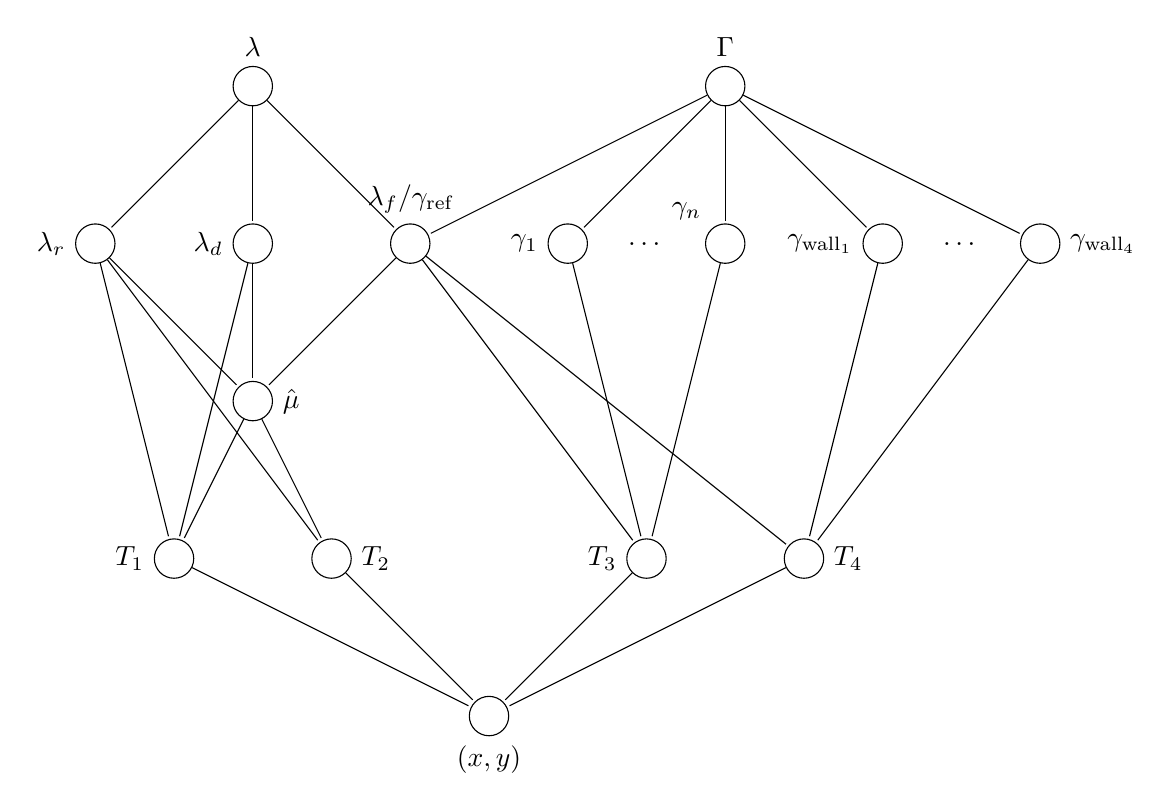
\begin{tikzpicture}[-, >=stealth', shorten >=1pt, auto, node distance=2cm, every state/.style={fill=white, draw=black, text=black, minimum size=0.5cm}]
	\node[state, label=above:$\lambda$] (cmd) {};
	\node[state, label=above:$\Gamma$] (world) [right of=cmd, xshift=4cm] {};
	\node[state, label=left:$\lambda_d$] (dist) [below of=cmd] {};
	\node[state, label=left:$\lambda_r$] (dir) [left of=dist] {};
	\node[state, label=above:$\lambda_f/\gamma_{\refobj}$] (ref) [right of=dist] {};
	\node[state, label=left:$\gamma_1$] (obj1) [below of=world, xshift=-2cm] {};
	\node[state, label=above left:$\gamma_n$] (objn) [right of=obj1] {};
	\node[state, label=left:$\gamma_{\textmd{wall}_1}$] (wall1) [right of=objn] {};
	\node[state, label=right:$\gamma_{\textmd{wall}_4}$] (wall4) [right of=wall1] {};
	\node[state, label=right:$\hat{\mu}$] (mu) [below of=dist] {};
	\node[state, label=left:$T_1$] (t1) [below of=mu, xshift=-1cm] {};
	\node[state, label=right:$T_2$] (t2) [right of=t1] {};
	\node[state, label=left:$T_3$] (t3) [right of=t2, xshift=2cm] {};
	\node[state, label=right:$T_4$] (t4) [right of=t3] {};
	\node[state, label=below:${(x, y)}$] (pt) [below of=t2, xshift=2cm] {};
	
	\path (cmd) edge (dist)
	         (cmd) edge (dir)
	         (cmd) edge (ref)
	         (world) edge (ref)
	         (world) edge (obj1)
	         (world) edge (objn)
	         (world) edge (wall1)
	         (world) edge (wall4)
	         (obj1) -- node[auto=false]{\ldots} (objn)
	         (wall1) -- node[auto=false]{\ldots} (wall4)
	         (dir) edge (mu)
	         (dist) edge (mu)
	         (ref) edge (mu)
	         (dir) edge (t1)
	         (dir) edge (t2)
	         (dist) edge (t1)
	         (mu) edge (t1)
	         (mu) edge (t2)
	         (ref) edge (t3)
	         (ref) edge (t4)
	         (obj1) edge (t3)
	         (objn) edge (t3)
	         (wall1) edge (t4)
	         (wall4) edge (t4)
	         (t1) edge (pt)
	         (t2) edge (pt)
	         (t3) edge (pt)
	         (t4) edge (pt);


\end{tikzpicture}
\end{center}

Given these features, we obtain the log-linear model
\[
\mathbb{P}_w(x, y|\lambda, \Gamma) = \frac{1}{z_w(\lambda, \Gamma)}\exp\bigg(\sum_{c = 1}^4w_cT_c(x, y|\lambda, \Gamma)\bigg)
\]
where $w$ is a vector of weights. We then learn the weights using MLE estimation.

\subsubsection{MLE Estimation for Learning Weights}
We trained the model using the data from scene \#1. We assume each data point is an iid sample from $\prob_w(x, y|\lambda, \Gamma)$. Let the 12 commands be specified by $\lambda^{(1)}, \ldots, \lambda^{(12)}$. For each command we collected 10 data points. Let $X$ represent all the data and let $X^{(i)}_j$ be the $j$-th data point for the $i$-th command. Then the joint probability of the data points can be expressed as

\begin{equation*}
\begin{split}
\prob_w(X|\lambda^{(1)}, \ldots, \lambda^{(12)}, \Gamma) &= \prod_{i = 1}^{12}\prod_{j = 1}^{10} \frac{1}{z_w(\lambda^{(i)}, \Gamma)}\exp\bigg(\sum_{c = 1}^4w_cT_c(X^{(i)}_j|\lambda^{(i)}, \Gamma)\bigg) \\
&= \bigg(\prod_{i = 1}^{12}\prod_{j = 1}^{10} \frac{1}{z_w(\lambda^{(i)}, \Gamma)}\bigg)\bigg(\prod_{i = 1}^{12}\prod_{j = 1}^{10}\exp\bigg(\sum_{c = 1}^4w_cT_c(X^{(i)}_j|\lambda^{(i)}, \Gamma)\bigg)\bigg) \\
&= \bigg(\prod_{i = 1}^{12}\prod_{j = 1}^{10} \frac{1}{z_w(\lambda^{(i)}, \Gamma)}\bigg)\exp\bigg(\sum_{c = 1}^4w_c\sum_{i = 1}^{12}\sum_{j = 1}^{10}T_c(X^{(i)}_j|\lambda^{(i)}, \Gamma)\bigg)
\end{split}
\end{equation*}

Our goal then is to find the argmax over $w$ of this function. This is the same as finding the argmin of the negative log, so we have
\begin{equation*}
\begin{split}
w^* &= \argmin_w -\log\prob_w(X|\lambda^{(1)}, \ldots, \lambda^{(12)}, \Gamma) \\
&= \argmin_w \sum_{i = 1}^{12}\sum_{j = 1}^{10}\log(z_w(\lambda^{(i)}, \Gamma)) - \sum_{c = 1}^4w_c\sum_{i = 1}^{12}\sum_{j = 1}^{10}T_c(X^{(i)}_j|\lambda^{(i)}, \Gamma)
\end{split}
\end{equation*}

This is the sum of exponential families, one for each $i, j$. Therefore the derivative with respect to $w_c$ of the log partition function is the expected value of the $c$-th feature. Therefore, 
\[
\frac{\partial}{\partial w_c} -\log\prob_w(X|\lambda^{(1)}, \ldots, \lambda^{(12)}, \Gamma) = \sum_{i = 1}^{12}\sum_{j = 1}^{10} \E_w[T_c(x, y|\lambda^{(i)}, \Gamma)] - \sum_{i = 1}^{12}\sum_{j = 1}^{10}T_c(X^{(i)}_j|\lambda^{(i)}, \Gamma)
\]

We use this to perform gradient descent. In order to calculate the probabilities and the partition function, we discretize the table with a grid of step size 0.1 inches. Once we do this, we have all the components necessary to calculate the gradient, and so we perform gradient descent until the gradient falls below a threshold level.

\section{Modeling Results}

We have successfully implemented this model in MATLAB and Python, and learned values of $w$ from the training data gathered in Experiment 1. Once trained using the MLE code implemented in MATLAB, our algorithm can parse a natural language command and, combined with information about the world $\Gamma$, produce a distribution over $(x, y)$ coordinates. Plotted below are distributions generated by the log-linear model with all four features enabled:

\begin{figure}
\centering
\begin{subfigure}{.5\textwidth}
  \centering
  \centerline{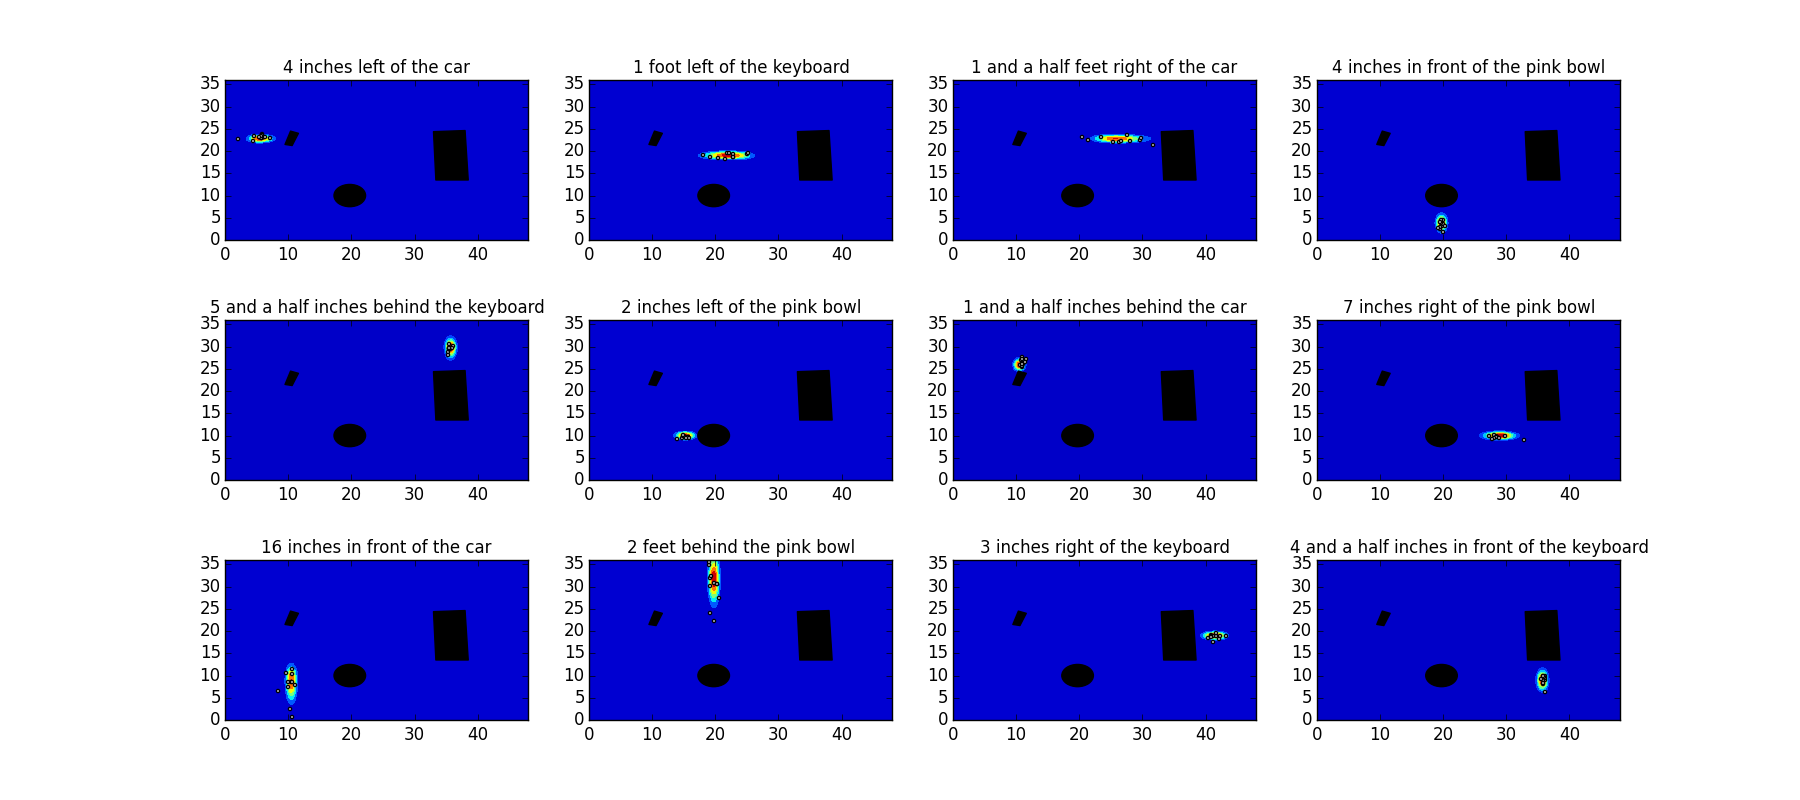
\includegraphics[scale=0.5]{images/all_commands_training.png}}
  \caption{ Distributions on training data}
  \label{fig:sub1}
\end{subfigure}
\begin{subfigure}{.5\textwidth}
  \centering
  \centerline{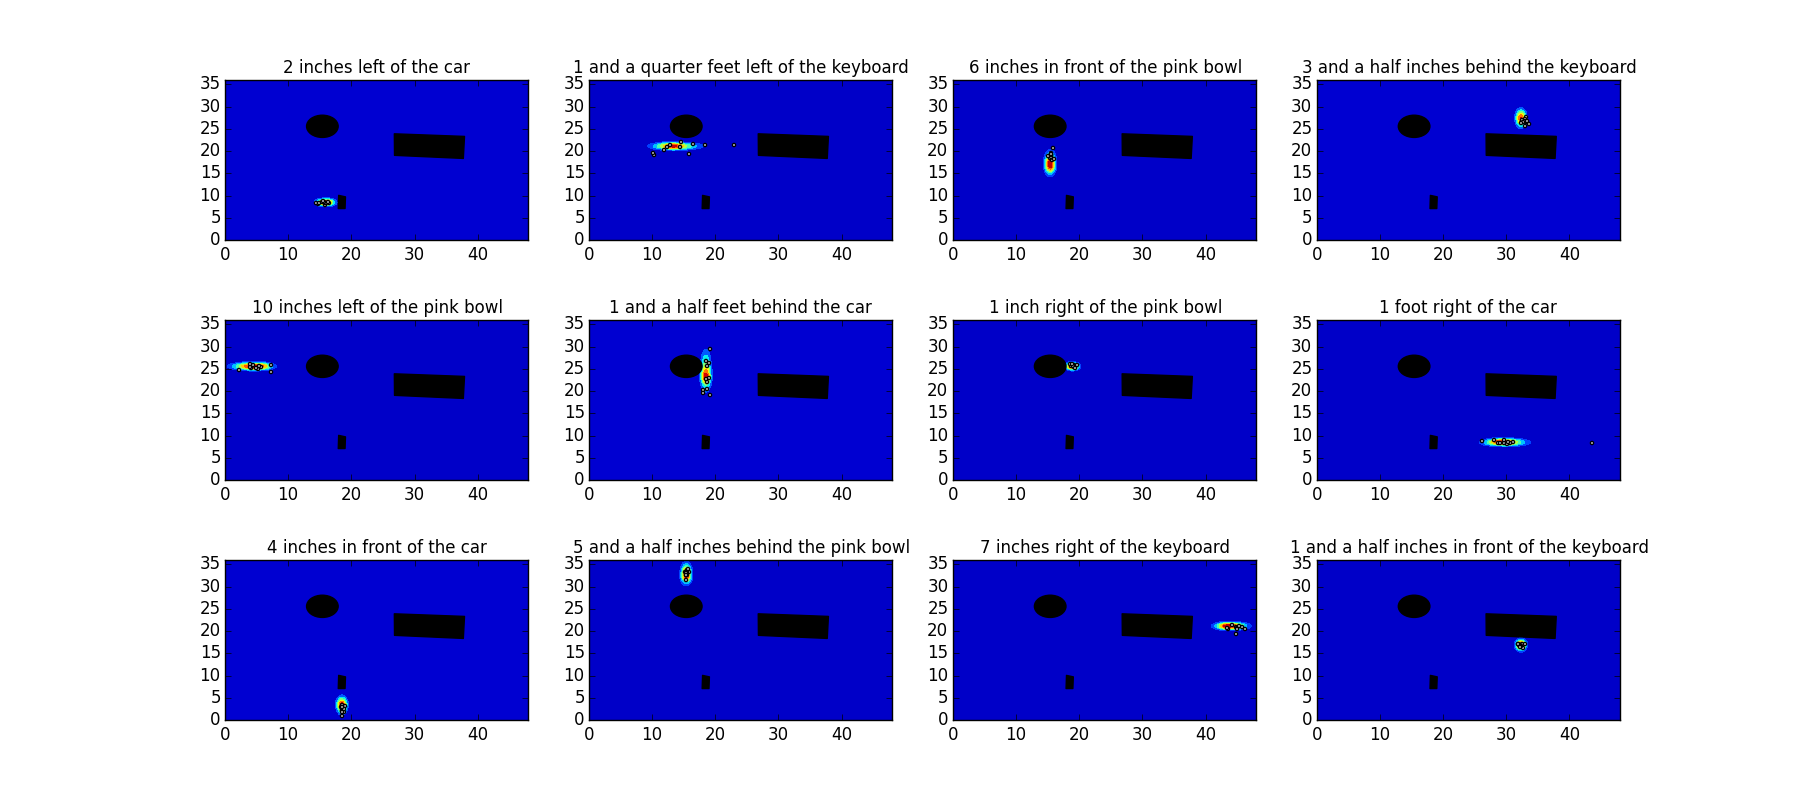
\includegraphics[scale=0.5]{images/all_commands_test.png}}
  \caption{Distributions on test data}
  \label{fig:sub2}
\end{subfigure}
\caption{Distributions from natural language commands and world information. Higher probability regions are in red.}
\label{fig:plot_distributions}
\end{figure}

\subsection{Algorithm Evaluation}

To evaluate the performance of our algorithm, we compared its performance to a baseline algorithm that fits a gaussian distribution around $\hat{\mu}$, the naive mean generated above. In addition, we compared it to log-linear algorithms trained and tested on subsets of our features, to determine the relative performance of different feature selections. All of these algorithms were compared to an empirical Gaussian distribution generated from the data in question - i.e. fitting a Gaussian to data for the specific $\lambda, \Gamma$ pair. In the following evaluation metrics, "empirical mean" and "empirical standard deviation" refer to the mean and standard deviation of this distribution. This is distinct from the baseline algorithm, where a Gaussian distribution is generated for a $\lambda, \Gamma$ using weights learned from the entire data set. We used three different performance metrics to evaluate our system: the distance between predicted and empirical means, and the combined log-probability of the data given our distributions, mean-squared error (MSE) of the algorithms on our data sets. Plots of these metrics are displayed below, followed by a discussion of their meaning. 

\begin{figure}[H]
\centering
\begin{subfigure}{.5\textwidth}
  \centering
  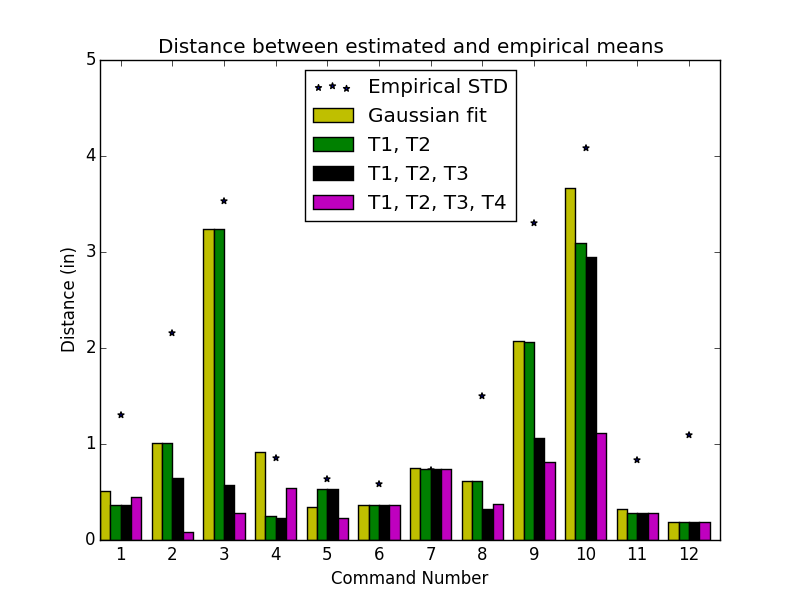
\includegraphics[width=1.1\textwidth]{images/mean_dist_training.png}
  \caption{Training data}
  \label{fig:sub1}
\end{subfigure}%
\begin{subfigure}{.5\textwidth}
  \centering
  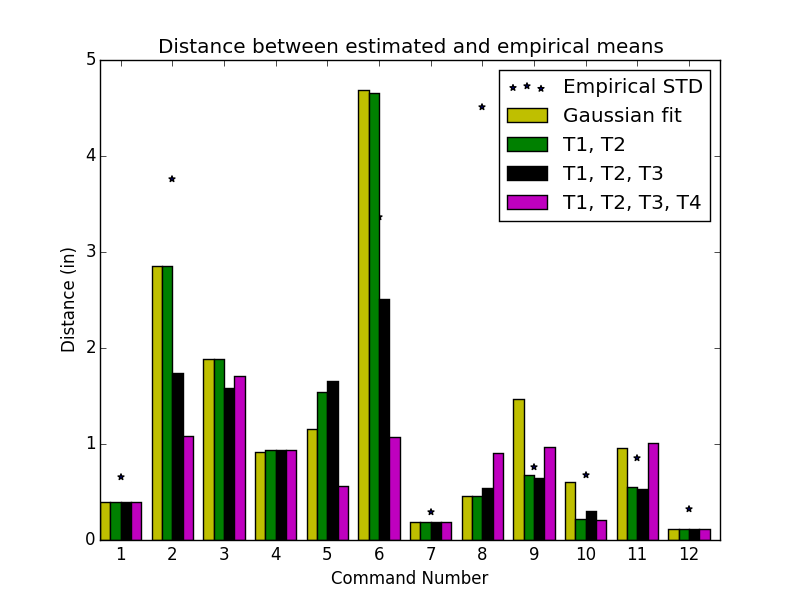
\includegraphics[width=1.1\textwidth]{images/mean_dist_test.png}
  \caption{Test data}
  \label{fig:sub2}
\end{subfigure}
\caption{Distance between empirical and predicted mean for all NL phrases. }
\label{fig:means}
\end{figure}

\begin{figure}[H]
\centering
\begin{subfigure}{.45\textwidth}
  \centering
  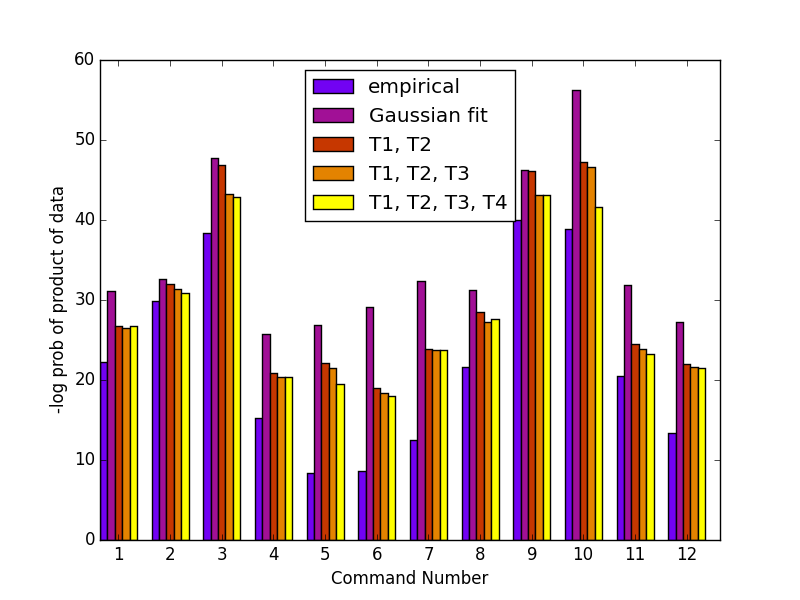
\includegraphics[width=1.1\textwidth]{images/logprob_training.png}
  \caption{Training data}
  \label{fig:sub1}
\end{subfigure}%
\begin{subfigure}{.45\textwidth}
  \centering
  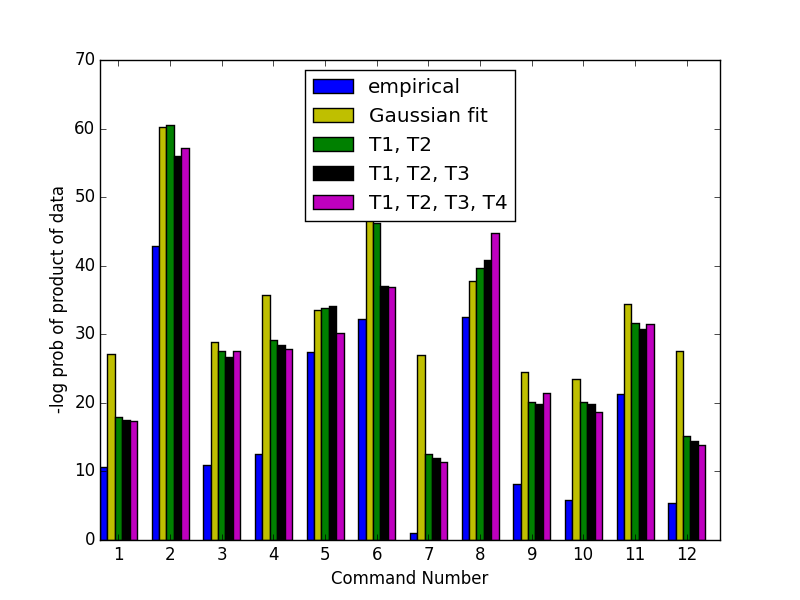
\includegraphics[width=1.1\textwidth]{images/logprob_test.png}
  \caption{Test data}
  \label{fig:sub2}
\end{subfigure}
\caption{Negative log probability of algorithms for all NL phrases}
\label{fig:logprob}
\end{figure}

\begin{figure}[H]
\centering
\begin{subfigure}{.5\textwidth}
  \centering
  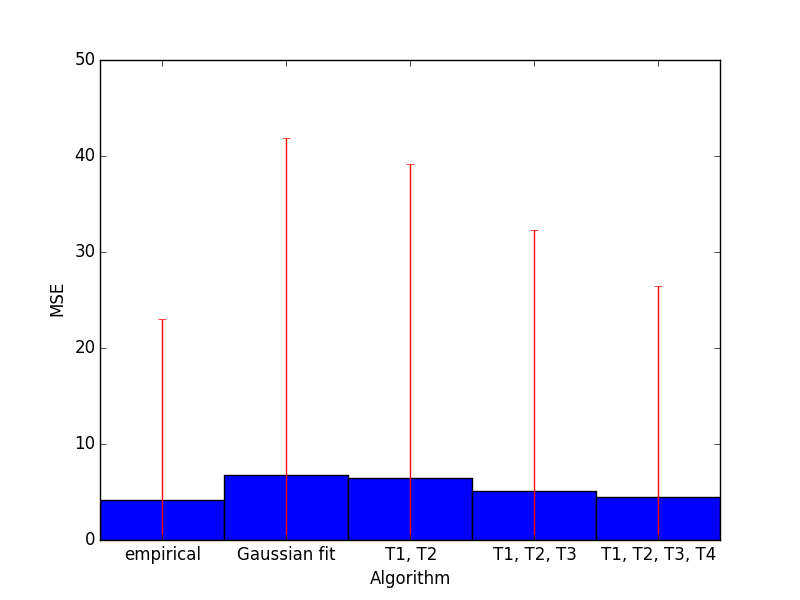
\includegraphics[width=1.1\textwidth]{images/mse_training.png}
  \caption{MSE across all training data}
  \label{fig:sub1}
\end{subfigure}% 
\begin{subfigure}{.5\textwidth}
  \centering
  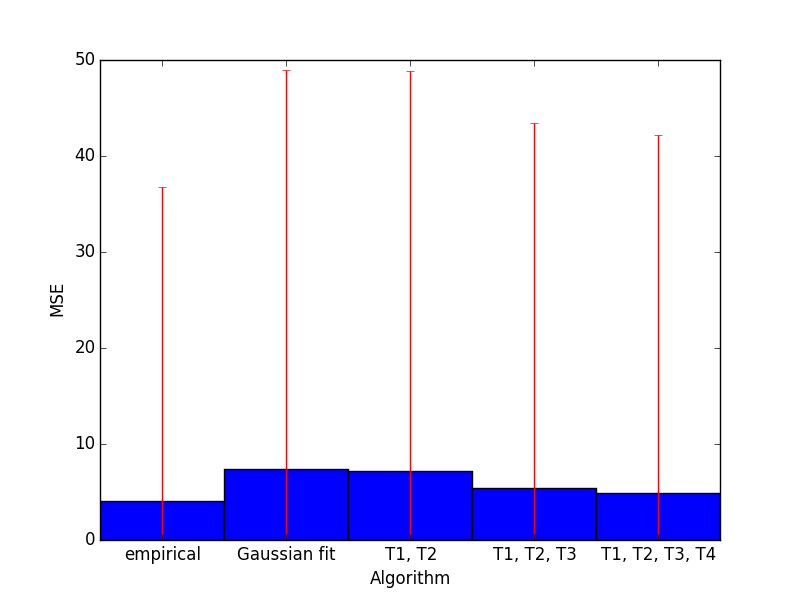
\includegraphics[width=1.1\textwidth]{images/mse_test.png}
  \caption{MSE across all test data}
  \label{fig:sub2}
\end{subfigure}
\caption{Mean-squared error by feature set. Confidence interval is twice the standard deviation of the squared error.}
\label{fig:mse}
\end{figure}

\subsection{Discussion of Results}

These evaluation metrics lead to two primary conclusions about the performance of the algorithm and possible avenues for future research. The first, and most obvious, conclusion can be derived from the command-wise plots: the performance of different feature sets, as well as the relative performance between algorithms using different feature sets, varies across commands. This is entirely logical and consistent with the algorithms' design - in cases where objects and walls in $\Gamma$ have minimal effect, the algorithms including T3 and T4 hinge losses would be expected to perform similarly to the gaussian fit and algorithms only using the first two features. As well, in commands with short distances, the distance term in feature T1 has little effect on the variance of the distributions. However, in commands with larger distances, the non-Gaussian log-linear models have a superior performance. Overall, the larger feature sets maximize log-probability of the data, although the distance between the empirical and predicted mean varies across the commands. For nearly every command, the predicted mean is within one standard deviation of the empirical mean. A notable exception is command 4 in the test data. In that case, participants expressed confusion about reference points on the object, due to duct tape used to secure the object to the whiteboard. 

The second conclusion derives from the MSE evaluation. As shown in Figure \ref{fig:mse}, increasing the size of the feature sets lowers the mean-squared error across all distributions. However, the confidence interval with p=0.95 shows that the MSE of every feature set is statistically indistinguishable. Given that we only have 10-12 data points per $\lambda, \Gamma$ pair, a large confidence interval is to be expected. In particular, the magnitude of the standard deviation is similar to that of the empirical distribution, demonstrating that the algorithms perform similarly in that regard. Even so, the small data sets do not allow a definitive conclusion on the relative performance of each feature set. While the complete feature set does look promising in regards to log-probability, distance between predicted and empirical means, and MSE, we cannot definitively say that the performance of the log-linear model with all features is superior to Gaussian or log-linear models with smaller feature sets. Discussion of how we plan to resolve this issue, and expand the capabilities of our model, is included below.

\section{Future Research}

\subsection{Gathering Data}

The limitations of our current model suggest multiple avenues for future research. The first is dramatically increasing the size of our data set, both in terms of $\lambda, \Gamma$ pairs and number of data points gathered per pair. This will reduce statistical variation in the training and test sets, and provide a larger set of training data so more accurate weight vectors can be gathered. With a sufficiently large data set, we could use cross-validation to train our model instead of merely using a training and test set. A larger data set will also provide insight into other factors affecting human behavior, allowing us to add more features or parameters to the model if necessary. We plan to investigate the use of Amazon Mechanical Turk to rapidly gather large data sets, if the tradeoffs (especially the lack of spatial grounding in relation to performing in-person experiments) are not too great. 

\subsection{Frames of Reference}

\subsubsection{Introduction}

One such factor is the use of multiple reference frames and reference points on objects with off-axis rotations. As mentioned in Experimental Resultss, humans possess multiple reference frames in which they can refer to objects, such as the relative frame, which contains directions relative to the speaker's orientation, and the intrinsic frame, where directions are defined based on inherent properties of the object. (Levinson 2001) For instance, a car might be placed in any position relative to the speaker, but the speaker has some knowledge of what the ``front" of the car should be regardless of its orientation. As well, we observed in experiments 3 and 4 (See Figure \ref{fig:refpts} for an example) that objects with off-axis rotations cause human subjects to vary which reference point on they object they use, even if they operate within the relative reference frame. The data points for these objects appears to separate into distinct clusters, suggesting that humans make a decision between discrete reference points and reference frames before choosing a point. 

\subsubsection{Mathematical Approach}

We plan to use a multi-peaked log-linear distribution to more accurately model this situation, by modifying features T1 and T2 to accept arbitrary frames of reference, direction vectors, and reference points. These latent variables will be generated from knowledge of the object's pose in the world $\gamma$, as well as inherent properties of the object for determining directions relative to intrinsic reference frame. Determining how to gather these object properties is largely a vision and object recognition problem. With a knowledge of the distribution of reference points $\rho$ and direction vectors $\vec{v}$, we can then marginalize over the joint probability $\prob(x, y | \lambda,\Gamma, \rho, \vec{v} )\prob(\rho, \vec{v} | \lambda, \Gamma)$ to produce a multi-peaked distribution. 

\[
\sum_{\rho, \vec{v}} \prob(x, y | \lambda,\Gamma, \rho, \vec{v} )\prob(\rho, \vec{v} | \lambda, \Gamma) = \prob(x, y | \lambda, \Gamma)
\]

However, we do not possess enough data about the relationships between objects, reference frames, and reference points to accurately model the distribution $\prob(\rho, \vec{v} | \lambda, \Gamma)$. A large part of the data collection described above will be gathering enough data to accurately model this relationship. We are evaluating an Attentional Vector Sum (AVS)-like approach (Regier and Carlson 2001) to generating direction vectors from frames of reference and reference points, but we will have to determine how to adapt their algorithm to our situation. 

\subsection{Improved Parsing}

We also plan to pursue a better model of the relationship between space and language by developing more advanced parsing capabilities. To simplify our parser, we restricted the language used to a standardized format when conducting our experiments. However, humans can use a variety of natural language phrases when describing points in space. We plan to perform ``inverted" versions of our experiments, where humans are given a point in space and asked to describe it using natural language. From there, in combination with linguistic and psychological research on this subject, we can begin to develop a parser that more accurately captures a mapping between natural language and spatial relationships. 

\section{Conclusion}
In this project we developed a log-linear model, which relates natural language commands to distributions of points in 2D space. We created an experimental procedure to determine how humans interpret these natural language commands. Our model takes in a subset of our data, and via maximum likelihood estimation, finds the feature weights. The model obtains promising results in terms of MSE and log probability of the data, but ultimately we have too little data to be conclusive either way. There are some phenomena that the model does not support, such as rotated objects. We hope to address this using a multi-peaked model built from our current one. In addition, our limited amount of data is a major constraining factor. We hope to address this either by performing more experiments or by moving to a platform such as Mechanical Turk.

\end{document}
